\chapter{Metodologi}
\section{Metode Penelitian}
\par
Penelitian ini merupakan penelitian teoretis dengan pendekatan analitis yang diawali melalui studi literatur mengenai keterbelitan pada sistem tiga-qubit. Analisis difokuskan pada formulasi matematis matriks koefisien sebagai ukuran keterbelitan, kemudian dilanjutkan dengan penerapan matriks koefisien pada keadaan kelas GHZ, kelas W, dan keadaan lainnya. Seluruh kajian dilakukan secara analitis tanpa melibatkan simulasi numerik maupun eksperimen.

%\section{Waktu Penelitian}
%Waktu pelaksanaan pengerjaan tesis dimulai pada awal semester genap 2025/2026 selama 6 bulan sejak bulan Januari 2026 sampai dengan bulan Juni 2026. Tempat dilaksanakannya tugas akhir ini adalah di laboratorium fisika teori (LaFTiFA) Departemen Fisika FSAD ITS Surabaya. Untuk jadwal pelaksanaannya ditunjukkan pada tabel berikut ini:

%\begin{figure}
 %  \centering
 %  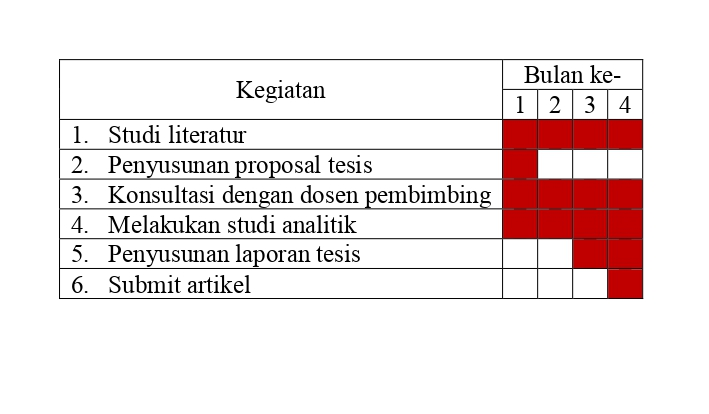
\includegraphics[scale=0.9]{Waktu.jpg}
 %  \caption{Waktu Penelitian}
 %  \label{waktupenelitian}
%\end{figure}



%\newpage
\section{Diagram Alir}
Penelitian ini merujuk pada diagram alir yang ditunjukkan oleh Gambar \ref{flowchart}.
\begin{figure}
   \centering
   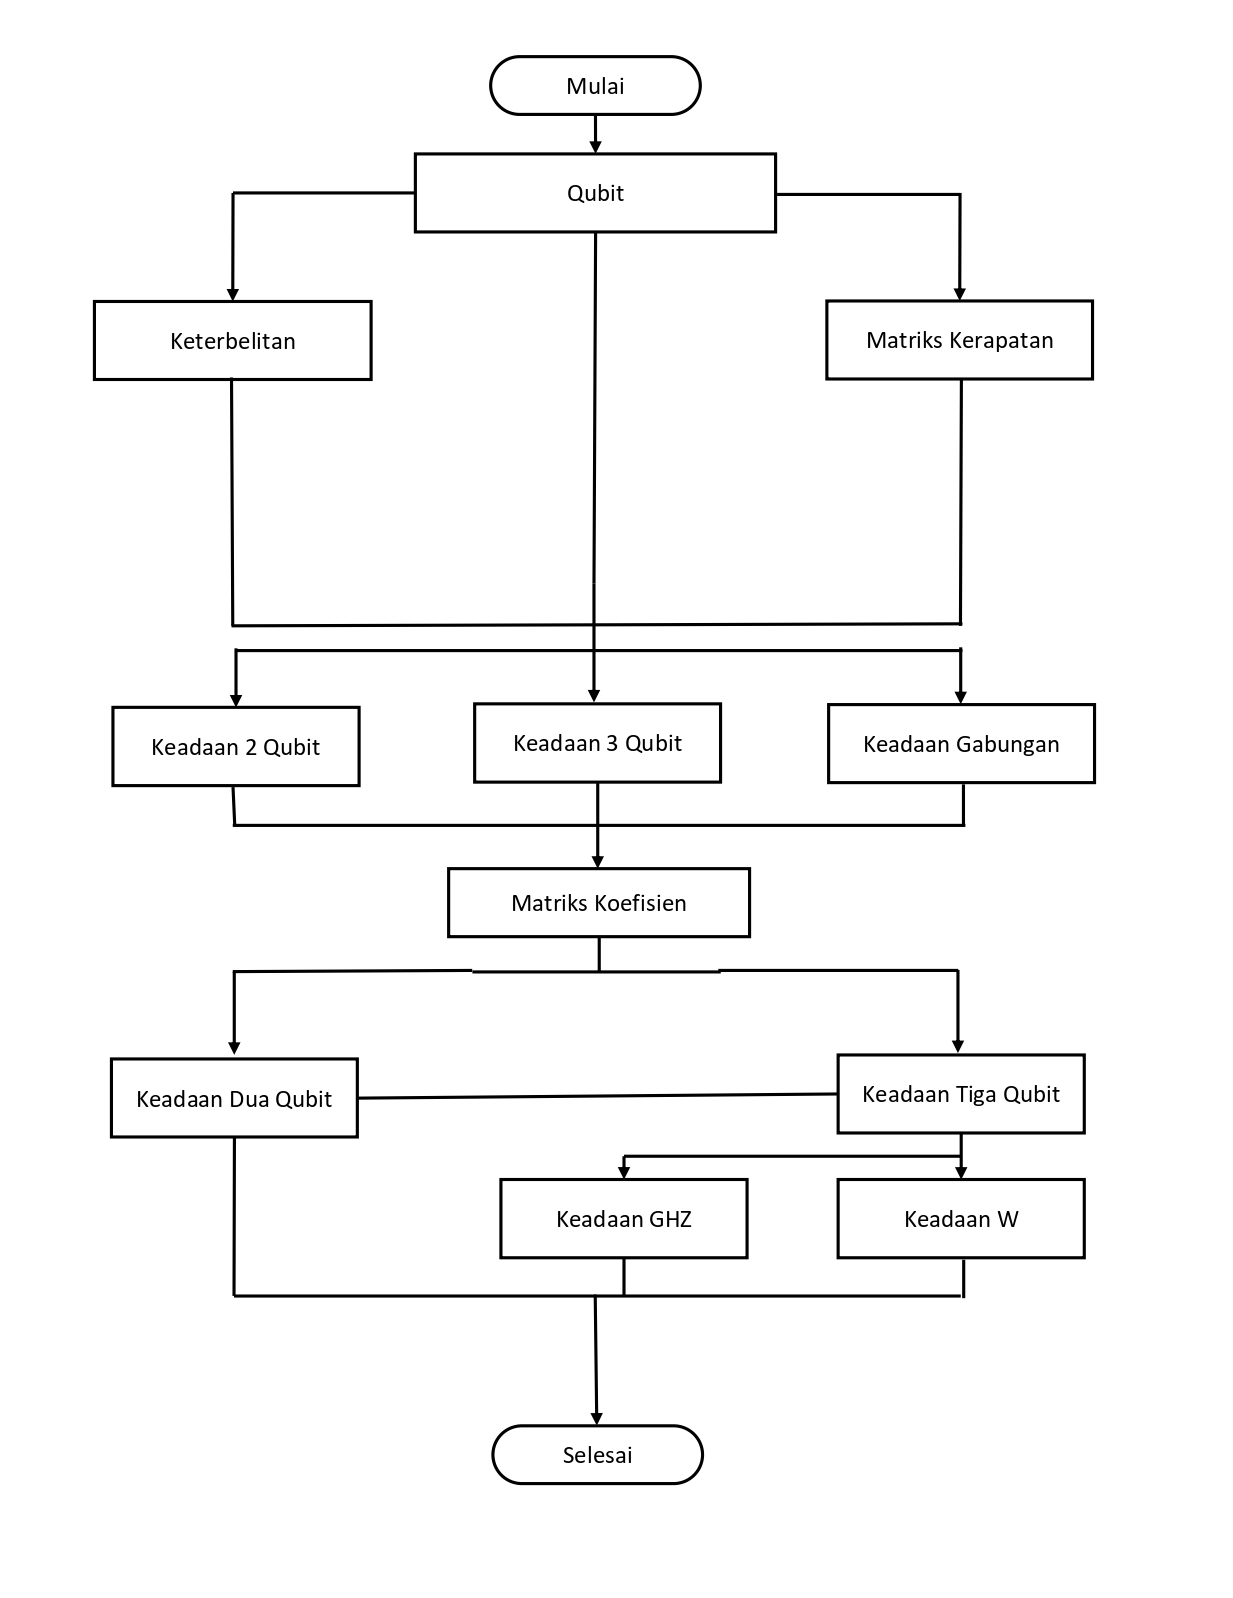
\includegraphics[scale=0.8]{FlowchartPraTesis.jpg}
   \caption{Diagram Alir Penelitian}
   \label{flowchart}
\end{figure}

%\newpage
%\thispagestyle{empty}
%\begin{center}
%	\topskip0pt
%	\vspace*{\fill}
%	\textit{\textbf{"Halaman ini sengaja dikosongkan"}}
%	\vspace*{\fill}
%\end{center}
%\pagebreak